\documentclass[12pt,a4paper,twoside]{article}
\usepackage{graphicx,fancyhdr}

%\pdfpagebox=4

\setlength{\parindent}{0cm}
\setlength{\parskip}{2ex plus1ex minus 0.5ex}

\addtolength{\evensidemargin}{-2.5cm}
\addtolength{\oddsidemargin}{-0.5cm}
\addtolength{\textwidth}{3cm}

\addtolength{\headheight}{0.2cm}
\addtolength{\topmargin}{-2.5cm}
\addtolength{\textheight}{2.5cm}

% \newcommand{\source}[1]{\textbf{\verb^#1^}}}
\renewcommand{\_}{\texttt{\symbol{95}}}
\addtolength{\fboxsep}{0.1cm}
\newcommand{\param}[1]{\textit{\textrm{\textmd{#1}}}}
\newcommand{\codebar}{\rule{\textwidth}{0.3mm}}
\newcommand{\todo}{\textbf{TODO}}

\newlength{\codelen}
\newcommand{\code}[1]
{\begin{center}\fbox{\parbox{16cm}{\texttt{#1}}}\end{center}}

\newcommand{\mission}[1]{\item[#1:]}
% \newcommand{\mission}[1]{\texttt{#1}\hspace{3mm}}

\fancyhead{}
\fancyhead[RO,LE]{\thepage}
\fancyhead[LO,RE]{ROBOC Summer School Projects}
\fancyfoot{}
\pagestyle{fancy}
% \pagestyle{empty}

\setcounter{secnumdepth}{1}

\newenvironment{bulletlist}
{
	\begin{itemize}
	\addtolength{\itemsep}{-1mm}
	% \setlength{\itemsep}{0ex}
	\setlength{\parsep}{0ex}
}
{
	\end{itemize}
}

\newenvironment{alphalist}
{
	\begin{enumerate}
	\setlength{\itemsep}{0ex}
	\setlength{\parsep}{0ex}
	\renewcommand{\labelenumi}{(\alph{enumi})}
}
{
	\end{enumerate}
}

\newenvironment{numericlist}
{
	\begin{enumerate}
	\addtolength{\itemsep}{-1mm}
	% \setlength{\itemsep}{0ex}
	\setlength{\parsep}{0ex}
}
{
	\end{enumerate}
}

\usepackage{hyperref}
\begin{document}

\centerline{\textbf{\LARGE ROBOC Summer School Projects}}
\vspace{0.5cm}
\centerline{August 2010}
\centerline{Author: David Ingram}
\centerline{Revised: David Eyers (\texttt{David.Eyers@cl.cam.ac.uk})}

{ \parskip 1mm plus 1pt \tableofcontents }

\section*{Introduction}

All projects use Art mode in ROBOC.
The most difficult project is Racetrack; the others are all about
the same difficulty.

\newpage
\section*{Project preferences form}

{\Large
Name:\\[1mm]

Previous programming experience:\\[10mm]

1st choice:\\[1mm]

2nd choice:\\[1mm]

3rd choice:\\[1mm]
}
\newpage
\section{Paint program}

The aim of this project is to start with the sketch program, and
develop it into a more fully-featured painting program. Start by
adding a colour palette. When the user clicks on the palette, it
should change their drawing colour. Do a three colour palette
first (say black, red and white); then try a larger one. You
should use a loop to draw the larger palette, specifying colours
by number instead of name, to make the program shorter. You can
calculate which colour the user has clicked on from the coordinates,
and turn this into the colour number. You may want to add a display
of the current drawing ink colour. Here is an example palette:

\begin{center}
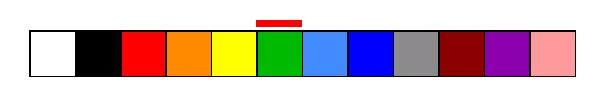
\includegraphics[scale=0.6,angle=0]{screenshots/artpixel/paint/palette}
\end{center}

Next, try adding a toolbox which lets the user select from different
drawing tools. For example you could let them draw lines, spots, squares,
stars, triangles, or with an italic pen nib. There could be a tool which
draws balloons using the \verb^image^ function. You could consider
different size tools, or an eraser or colour picker which changes the
drawing colour to one selected from the picture using \verb^examine(x,y)^.
Here is an example toolbox, and some different tools in use:
\begin{center}
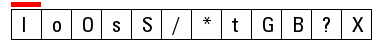
\includegraphics[scale=0.6,angle=0]{screenshots/artpixel/paint/toolbox}\\[2mm]
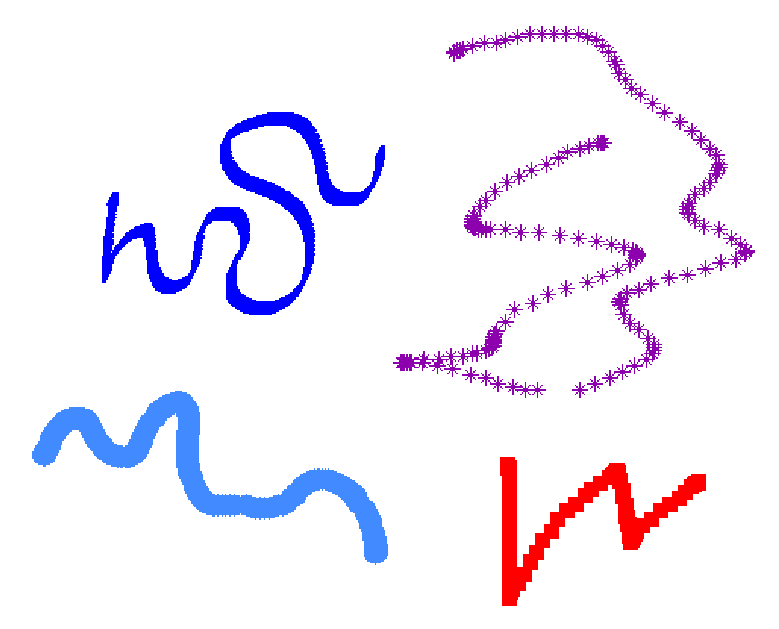
\includegraphics[scale=0.5,angle=0]{screenshots/artpixel/paint/tools}
\end{center}

\newpage
\section{Memory game}

This project is to write a memory game, in which playing cards (with
pictures of animals) are arranged on the screen. The player clicks
on two cards, which are turned over; if they match they are both removed,
otherwise they are hidden from view again. Play continues until there
are no cards left.

It is advisable to begin with some simpler programming tasks.
Write a function to print 48 playing card backs in a grid, using the
\verb^Card^ image. Then write a function to print 24 pairs of animals
in a grid (2 each of image numbers 0 to 23). Next, create an array
to hold the card numbers, and work out a way of using the
\verb^random(a,b)^ function to mix up the order. Display the
48 mixed up animals. Allow the user to click on cards; deduce
which card position has been clicked on and remove it from the
display. Then put this all together to make the game.

The left picture below shows the animals arranged in a grid during testing
(during the game they are never all shown at once, of course), before
the \verb^random^ function has been used to mix them up. The right picture
shows a typical situation during a real game, in which most of the cards
are face down, some pairs have already been removed, and the user has
just turned over two cards (which don't match, so these will be hidden
again next time they click the mouse).

\begin{center}
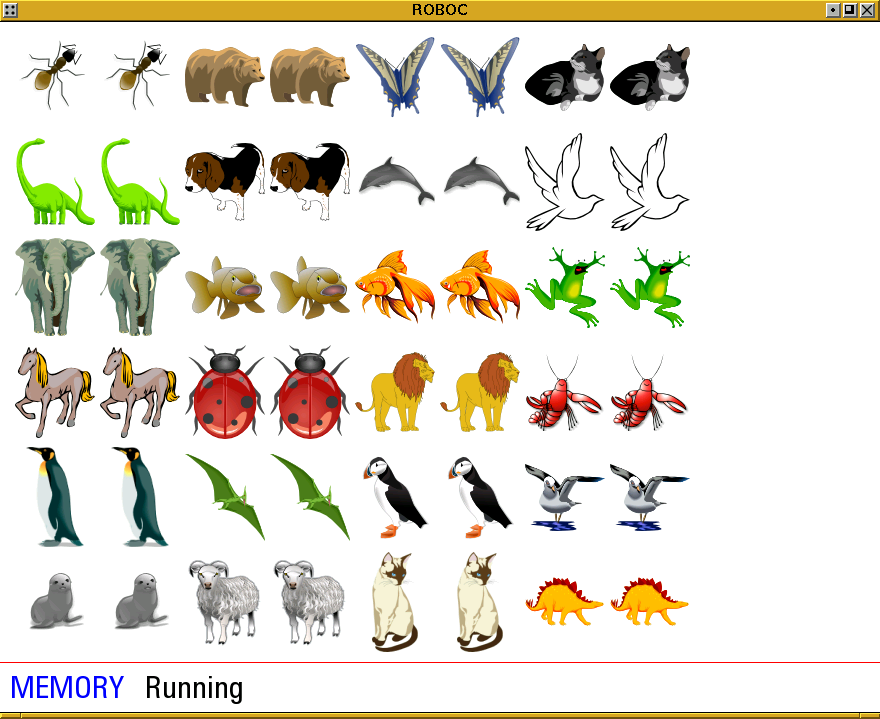
\includegraphics[scale=0.32,angle=0]{screenshots/artpixel/memory/animal_grid}
% 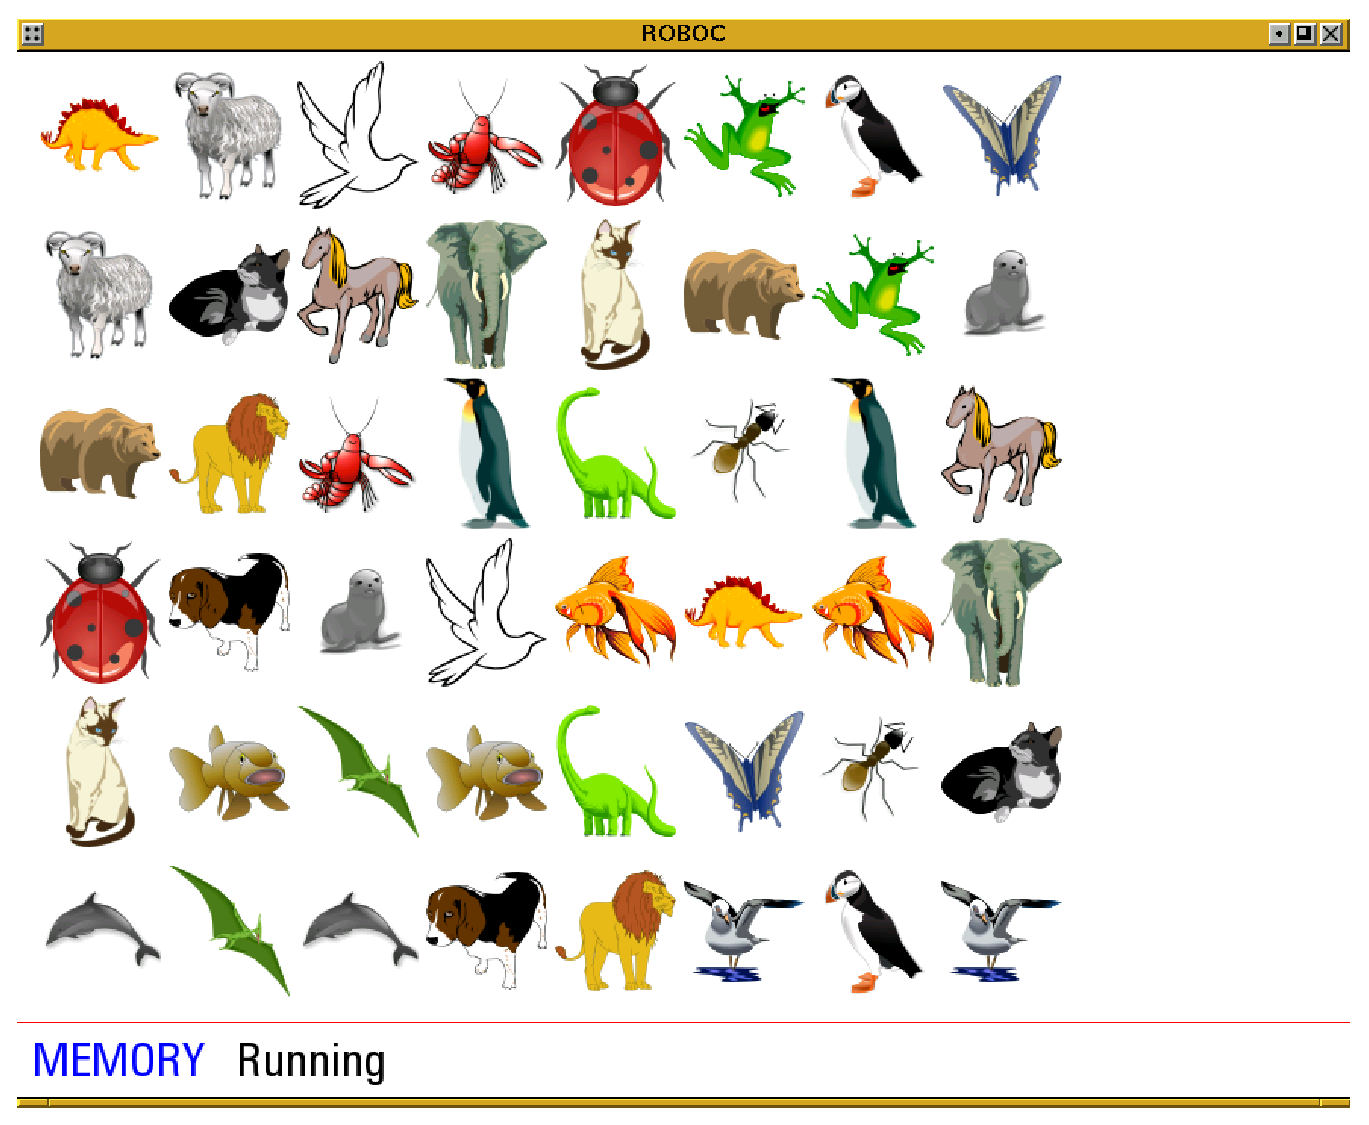
\includegraphics[scale=0.32,angle=0]{screenshots/artpixel/memory/animal_random.eps}\\
% 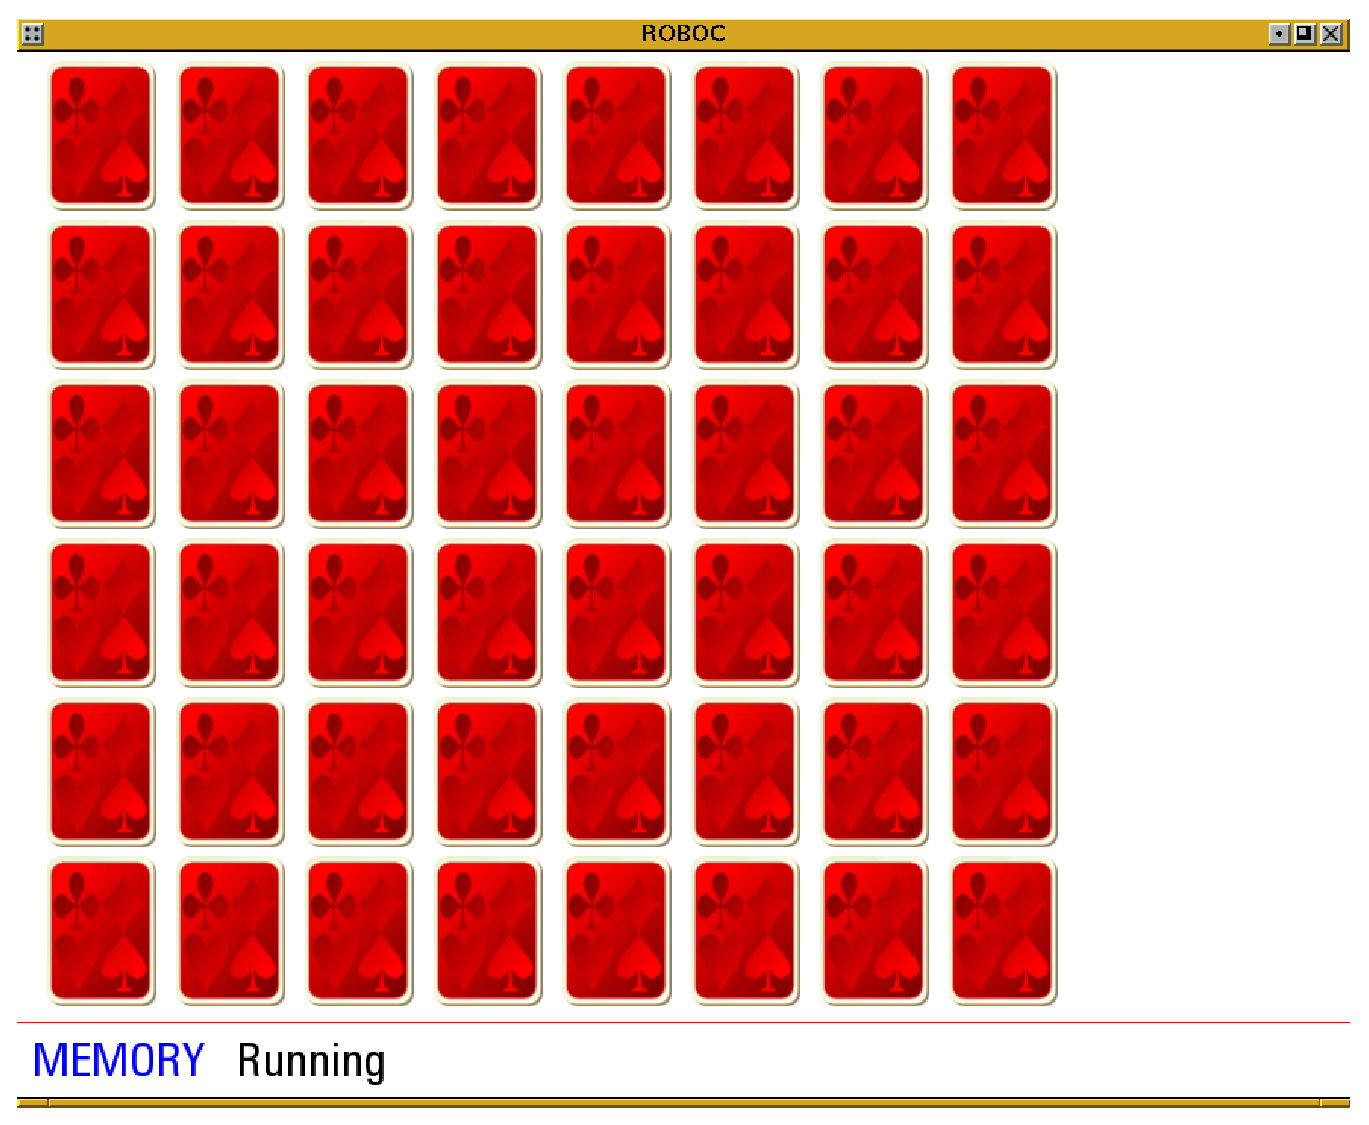
\includegraphics[scale=0.32,angle=0]{screenshots/artpixel/memory/card_backs.eps}
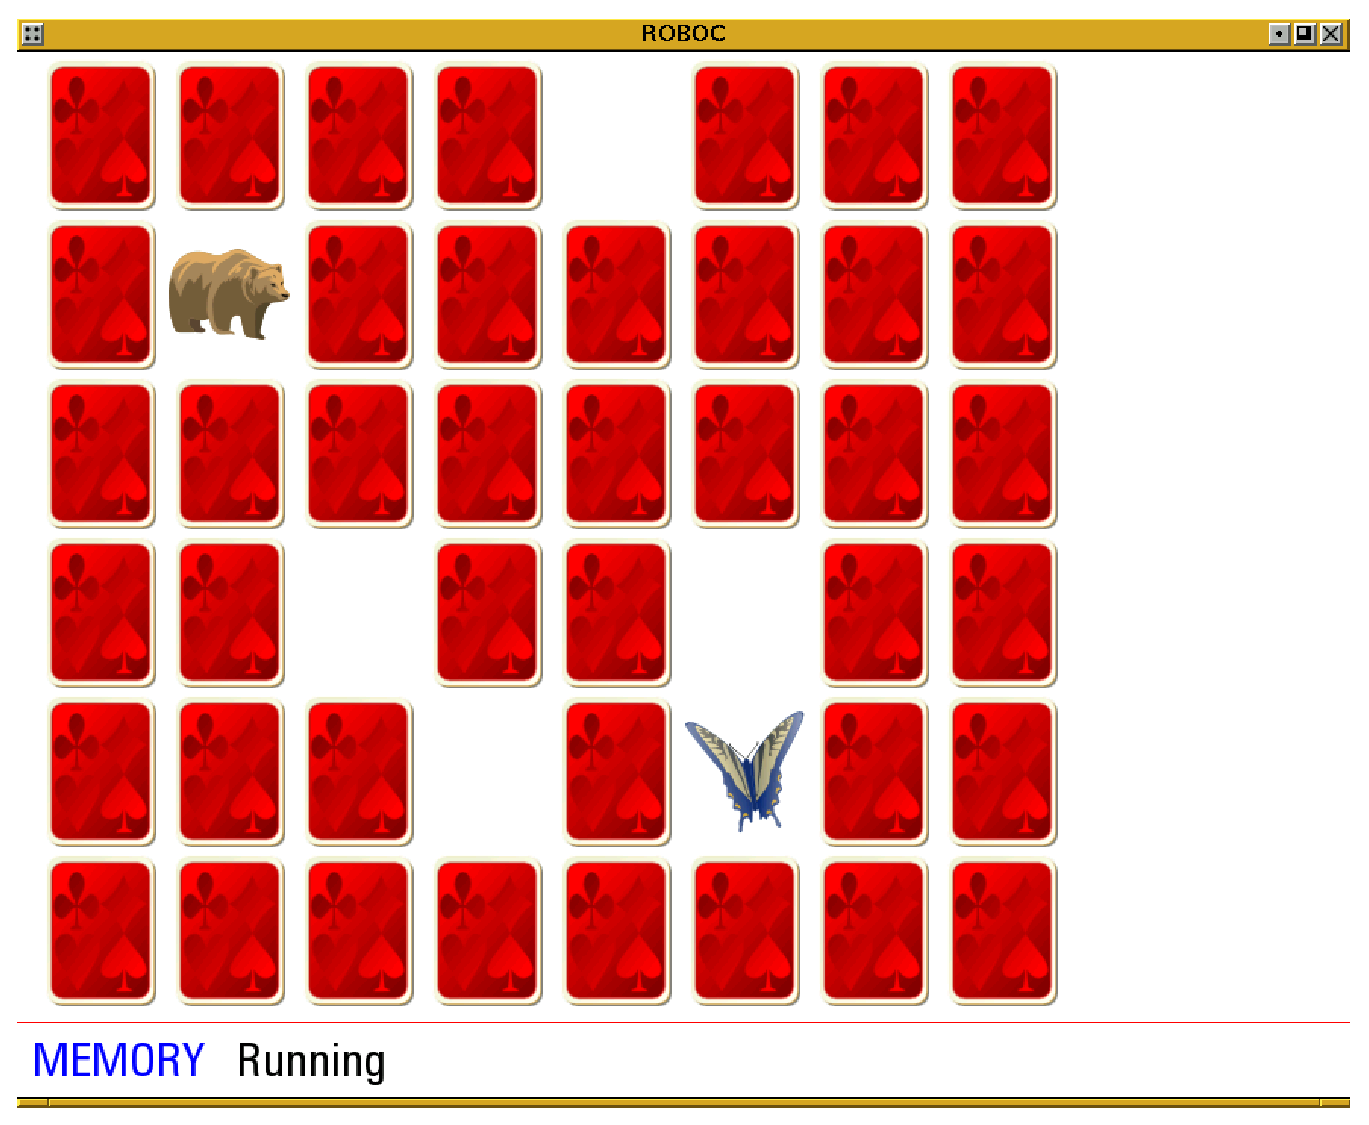
\includegraphics[scale=0.32,angle=0]{screenshots/artpixel/memory/playing}\\
% \begin{center}
% 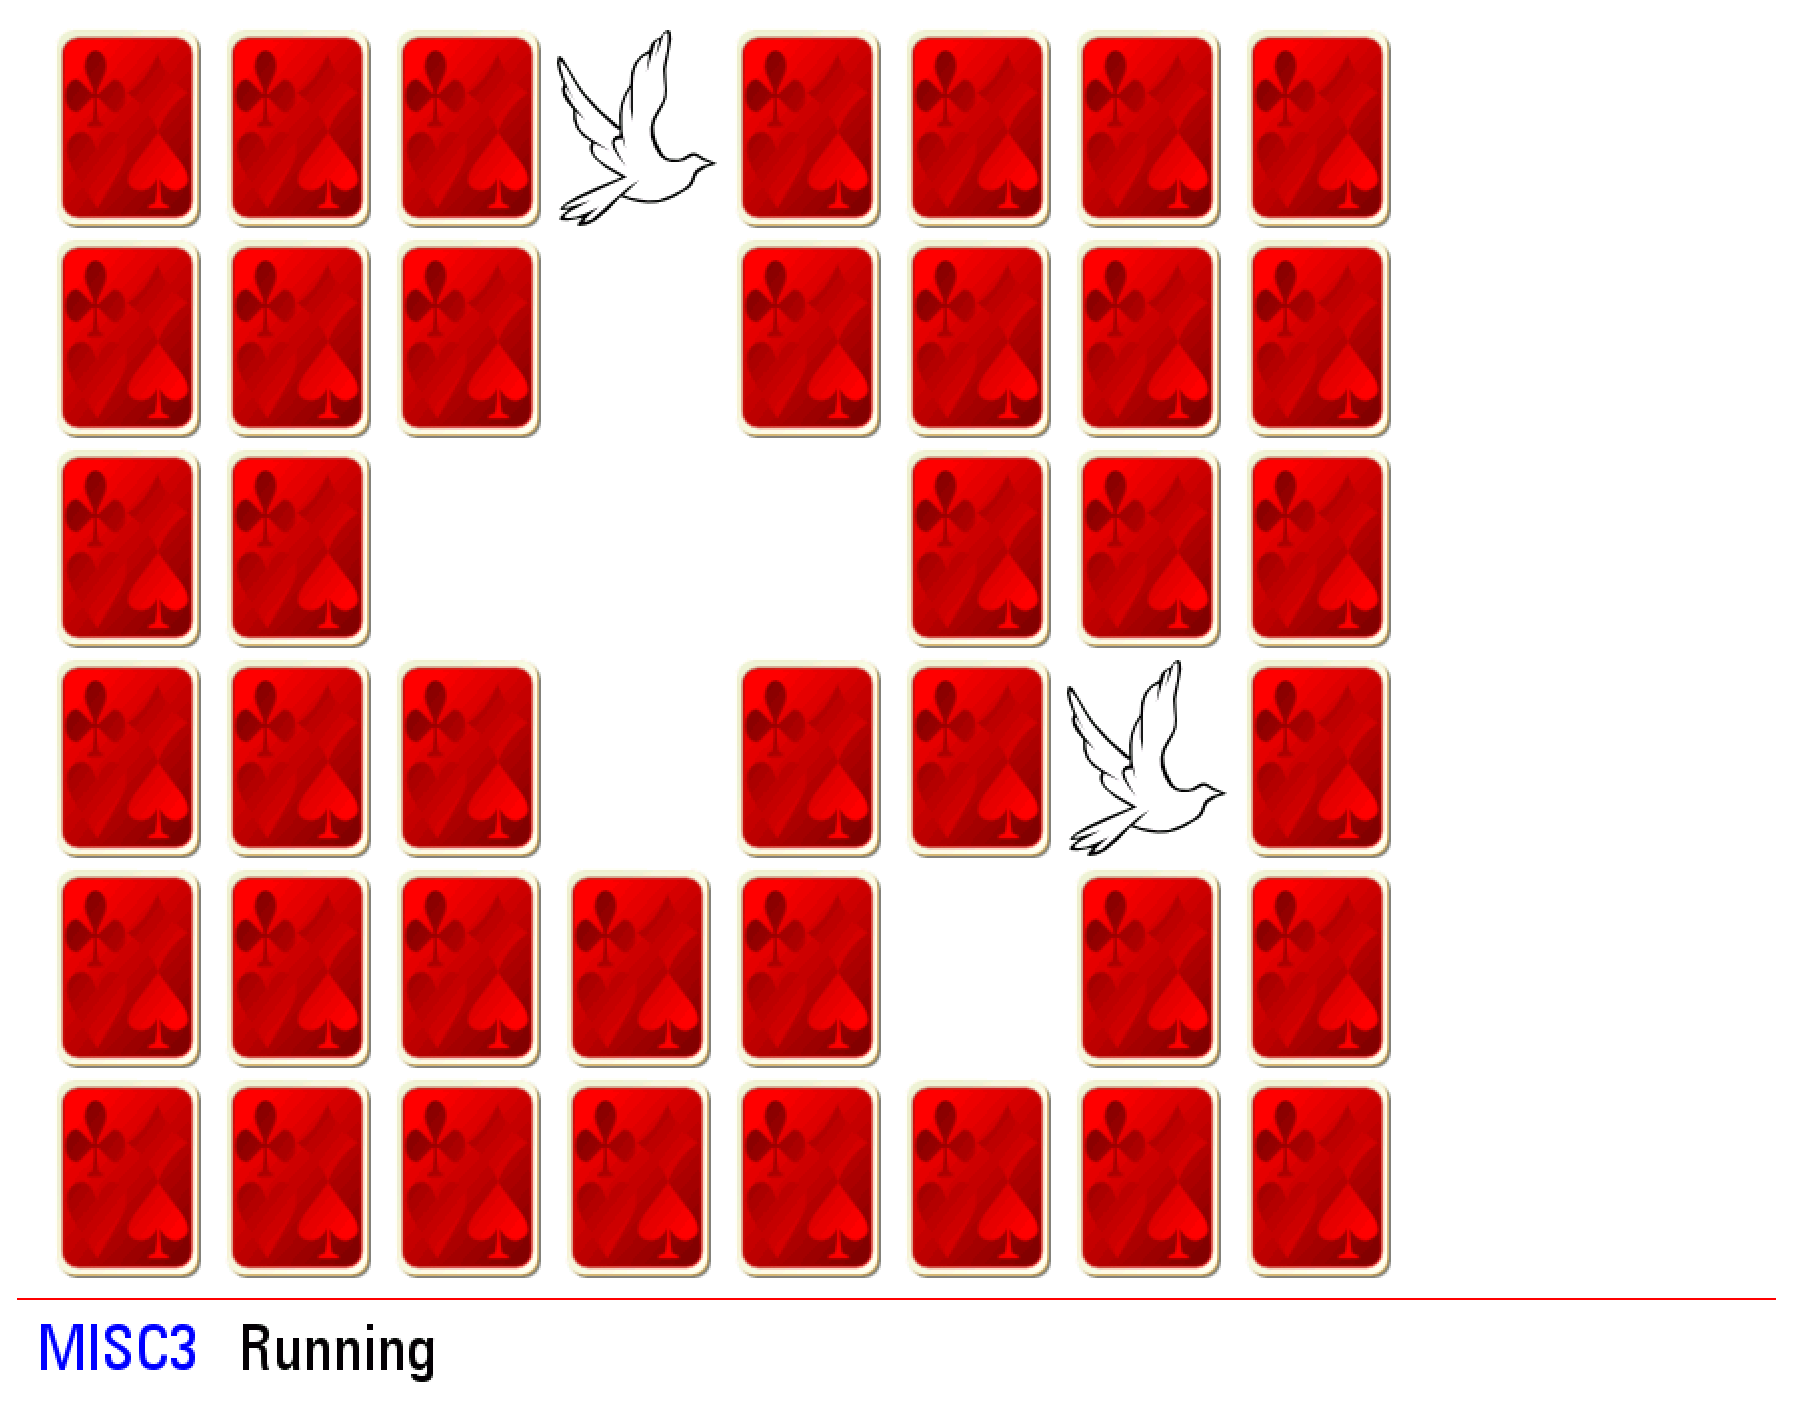
\includegraphics[scale=0.25,angle=0]{screenshots/artpixel/memory/snap.eps}
% \end{center}
\end{center}

\newpage
\section{Racetrack}

This project develops a simple car racing game. Start by calling
\verb^background "track"^ to display a racetrack. Now write a function
to display a small car somewhere on the track. To keep things simple
we are going to use a triangular car, like this:

\begin{center}
%\fbox{
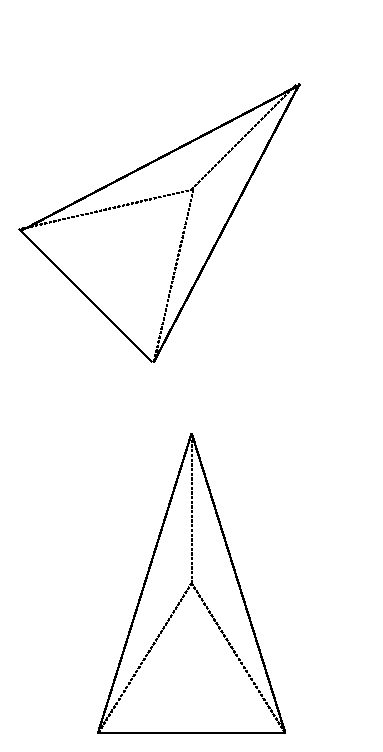
\includegraphics[scale=0.32,angle=-90,trim=20mm 20mm 145mm 140mm]{diagrams/car}
%}
\end{center}

The dotted lines give you an idea of how to calculate the positions
of the corners from the centre point. You will have to use \verb^sin^ and
\verb^cos^ functions of the appropriate angles. Once you have worked out
the positions of the corners, connect them with lines using the \verb^line^
function. Now create a function which can draw the car at any position
and facing in any direction, using parameters.

Look at the lander program from the example programs list to see how
to make a loop which understands key presses. Make your loop respond
to the left and right arrow keys by spinning the car anticlockwise
or clockwise in response. When the car's direction changes you will
need to erase the old car (by drawing it again but in white), then
call the draw function again with a different angle in the colour of the car.
Be sure to use
the same time delay code as the lander so that the program runs at
the correct rate, and doesn't go too fast.

Next add an accelerator key, and a key for reverse gear (only operable
from stationary). When the accelerator is pressed, the car should
speed up (create a variable to keep track of the current speed).
When the accelerator is not pressed, it should slow down gradually.
Again you will need to do some trigonometry based on the direction it
is facing to work out how to update its position.

Now we need to add a collision detection function. This should calculate
the positions of the three corners of the car, just like the draw car
function. It can then use the \verb^examine^ function to see if that
position is off the track or not. Call the collision detection function
every time the car moves or rotates. If the car is about to move off the
track, it should stay at its current position instead of moving, and
its speed should be immediately reduced to zero. The driver may
have to use reverse gear to back away from the wall before they have
room to turn around.

%\newpage
%\section{Robot navigation}
%
%In this project you will write a program to control an iRobot Create
%robot and help it navigate around the floor of the room. The robot
%is connected to a OLPC laptop which provides remote control from
%ROBOC. Human control
%is not allowed, so your program must steer around obstacles itself.
%You should run in Art mode but it is not necessary to draw anything
%on the screen.
%
%To control the robot, send network messages to the user \verb^robot^.
%Each message must contain a single letter; this can be \verb^a^
%to accelerate the robot forward, \verb^d^ to decelerate it,
%\verb^l^ to make it turn to the left or \verb^r^ to make it turn
%to the right. Two or three accelerates in a row will make it move faster.
%A message containing \verb^s^ can be used as an emergency
%start/stop from any speed.
%
%To find out if the robot has hit an obstacle, make sure your
%program includes\\
%\verb^self("controller")^\\
%You can then listen
%to \verb^NetEvent^ to receive collision messages. These will
%consist of either the letter \verb^L^ or \verb^R^ to indicate
%a crash on the left or right side of the robot's front
%bumper respectively. Make sure you tell the robot to stop
%immediately when it has had a collision!
%
%Your program should help your robot explore the area by diverting
%around objects in its path. During the project presentations you
%will be given a maze you have never seen before and the robot
%must get through it. The robot will always be positioned so that
%it starts facing directly torwards the goal and at a distance
%of exactly 5 metres, however.
%
%You may find it useful to keep
%track of time with the Art mode \verb^delay()^ and \verb^time()^
%functions, and work out how fast the robot travels and what
%angle it rotates by when turning on the spot. These can
%help you calculate how to get the robot back on target after
%it has to divert to avoid an obstacle.
%
%\newpage
%\section{3D pinball}
%
%This project is done in 3D mode, instead of Art mode.
%First create a rectangular pinball table with a moving ball
%on top of it. The ball's X and Y co-ordinates and
%horizontal and vertical speed need to be kept in global
%variables so that they are not reset each time the program
%runs to redraw the 3D scene. Hint: if you want to set some initial
%values for them, use another variable called \verb^setup^ which
%is initially 0 but gets set to 1 after the first run.
%
%Make the ball bounce off the four edges of the pinball table
%by reversing its velocity in the appropriate direction when it
%reaches the edge. Now
%tip the table by rotating about the X axis by 30 degrees,
%and program keyboard controls
%to adjust the tilt (say the 9 and 0 keys). You will need to
%listen to \verb^KeyPress^ events and use the \verb^poll()^
%function. Add gravity, the strength of which will depend on the current
%angle of the table. The effect of gravity is always to accelerate
%the ball down the Y axis. Also add some friction
%which gradually reduces the ball's Y-axis speed over time.
%
%Next make the 1 and 2 keys control two large flippers at the
%bottom of the table. These should move when the relevant
%key is pressed and return when it is released (using
%\verb^KeyRelease^). If the ball is near to the flipper when
%it moves it should be accelerated along the Y axis.
%
%Now consider obstacles for the ball to bounce off in
%the middle of the table. Can you create a row of bricks stored in
%an array, which
%disappear when the ball hits them, like in Breakout?

\newpage
\section{Shared whiteboard}

This project is to allow two users on different computers to participate
by drawing on the same canvas (so both users see the results of both
drawing on their screen). You should start with the sketch program,
and add networking. First use the \verb^send^ command to notify the other
computer when the user has clicked with the mouse. The other program
should add \verb^NetEvent^ to the event types it is listening to.
Initially you might arrange for it to display a shape in the
corner of the screen when the other user clicks with the mouse, just to
test the communication is working. Make it work in both directions.

Next you will need to encode the coordinates where the other user has
clicked within the network message it sends. You can use the string
join operator (\verb^:^) to do this, and the \verb^word(n, string)^
function at the other end to extract the information. If a text string
consists of just a number it is automatically converted to numeric form.
If the basic program works, can you encode the difference between
clicks and drags, or which mouse button was used?

This project only requires a short program to solve, but a significant
practical difficulty is making sure the programs on the two machines
you are using are kept up to date, and do the same things (there is
no automatic way to transfer a program to another computer).

% \section{Map tool}

\end{document}
